\section{Experiments}\label{s:exp}
In this section, we present the results of our experiments.  We execute \sys on $13$ datasets based on three sets of real-world cases---machine learning competitions, data analysis pipelines, and \company---and report accuracy measures and end-to-end runtime.  Then, we present a series of micro-benchmarks that evaluate each of the modules of \sys.  Our goal is to understand the conditions where automated cleaning is able to accurately detect and repair data in a way that improves the held-out test accuracy.

\subsection{Baselines and Methods}
To the best of our knowledge, there does not exist a comparable general purpose ML+Data Cleaning system to \sys in industry or academia.
We evaluate \sys against a number of baseline approaches inspired by solutions proposed in literature. 

\vspace{0.25em}\noindent\textbf{No Cleaning (NC): } We train a model without any modification to the training or test data.

\vspace{0.25em}\noindent\textbf{Quantitative (Q): } We train a model where only quantitative outliers in both training and test are imputed with a mean value. \ewu{Are outliers detected using isolation forest + numerical attribute featurizer?} 

\vspace{0.25em}\noindent\textbf{Integrity Constraint (IC): } We read through each dataset to identify a set of anomalous values for each attribute on a best-effort basis.  We then codified these as integrity constraint rules, and corrected the identified errors using a statistical distortion minimization metric as in~\cite{prokoshyna2015combining}.\ewu{  In one sentence what is the statistical distortion min metric}

\vspace{0.25em}\noindent\textbf{Quantitative + IC (Q+IC): } We use the quantitative and integrity constraints for detection; we use mean and mode imputation as repair functions for numerical and text attributes, respectively.

\vspace{0.25em}\noindent\textbf{Best Single (Best-1): } We run \sys with $B=1$ and identify the  single best conditional repair.

\vspace{0.25em}\noindent\textbf{Worst Single (Worst-1): } We run \sys with $B=1$ and identify the single worst conditional repair..

\stitle{BC-3: } We run \sys with $B=3$.

\stitle{BC-5: } We run \sys with $B=5$.


\vspace{0.25em}

\ewu{NEED TO EXPLAIN WHAT TEST DATASET IS.}


In all of our experiments, we used standard classification models and featurization techniques from Python \textsf{sklearn}.
The classifiers were trained in Python 2.7 and timing experiments were run on an Amazon EC2 m4.16xlarge instance\footnote{64 virtual cpus and 256 GiB memory}.
To avoid overfitting, we carefully designed the accuracy evaluation experiments for \sys by using a ``doubly'' held out test dataset: the test dataset used to optimize \sys is different from a completely unseen test dataset that is solely used to report the final prediction accuracy.
We describe hyper-parameter settings for each technique in the text of each experiment.

We used the \textsf{sklearn} Random Forest classifier with custom depth and branch parameters.  The training procedure uses a set of standard featurizers (hot-one encoding for categorical data, bag-of-words for string data, numerical data as is) in a similar fashion as~\cite{DBLP:conf/sigmod/GokhaleDDNRSZ14}.  Note that these featurizers are used as part of the black-box training procedure and are distinct from those used in the detector generator library.




\begin{table*}[t]
\centering
\label{tab:accuracy}
\begin{tabular}{|l|r|r|r|r|r|r|r|r|r|}
\hline
ML Competition& NC & Q &	IC & Q+IC &	Best-1 &	Worst-1 &	BC-3 & BC5 & Rel. Improvement\\
\hline
USCensus	&0.85&	0.82&	0.86&	0.84&	0.87&	0.79&	0.88&	\blue{0.91} & +4.5\% \\
Emergency &	0.67&	0.72&	0.67&	0.72&	0.72&	0.66&	0.72&	\blue{0.75} & +4.7\%\\
Sensor	&0.92&	0.93&	0.92&	0.89&	0.92&	0.8&	\blue{0.94}&	0.94 & +1.3\%\\
NFL	&0.74&	0.74&	0.76&	0.75&	0.76&	0.74&	0.79&	\blue{0.82}& +5.1\%\\
EEG	&0.79&	0.82&	0.79&	0.83&	0.83&	0.7&	0.85&	\blue{0.89}& +6.8\%\\
Titanic	&0.83&	0.72&	0.83&	0.76&	0.83&	0.69&	0.83&	\blue{0.84}& +1.1\%\\
Housing	&0.73&	0.76&	0.73&	0.77&	0.77&	0.65&	\blue{0.81}&	0.76& +5.1\% \\
Retail	&0.88&	0.88&	0.91&	0.91&	0.91&	0.87&	0.94&	\blue{0.95}& +4.3\% \\
\hline
\hline
Data Analytics & NC & Q &	IC & Q+IC &	Best &	Worst &	BC-3 & BC5 & Rel. Improvement\\
\hline
FEC  & 0.62 & 0.53 & 0.61 & 0.57 & 0.71 & 0.51 & 0.74 & \blue{0.77} &  +8.4\% \\
Restaurant (Multiclass) & 0.42 & 0.42 & 0.58 & 0.68 & \blue{0.62} & 0.36 & 0.61 & 0.60 & (1.61)\% \\
\hline
\hline
Company X & NC & Q &	IC & Q+IC &	Best &	Worst &	BC-3 & BC5 & Rel. Improvement\\
\hline
Dataset 1 (AUC) &0.60&0.59&0.60&0.60&0.61&0.59&0.66&0.69& +13\% \\
Dataset 2 (AUC) &0.55&0.53&0.52&0.55&0.55&0.52&0.61&0.63&\\
Dataset 3 (AUC) & & & & & & & & &\\
\hline
\end{tabular}
\caption{End-to-end accuracy results for each dataset and experimental method. We report standard classification accuracy.  The right column summarizes the accuracy improvement relative to the best non BC-3/5 approach.}
\end{table*}


\subsection{End-to-End Accuracy}
In our first experiment, we evaluated the accuracy of \sys compared to the baselines.
We tried to minimize hyper-parameter tuning as much as possible to simulate a real-scenario where extensive tuning and parameter search might be expensive.


\subsubsection{ML Competition Datasets}\label{exp:comp}
We downloaded 8 binary classification datasets from Kaggle competitions and benchmarks in the UCI ML repository.  \ewu{The next two sentences seem contradictory: they are clean, but dirty} These datasets are mostly clean as they have been extracted, structured, and published.
Nevertheless, they contain missing values, numerical outliers, and pattern errors (oddly formatted values).
For this set of experiments, we used a single hyper-parameter setting for all the detectors and classification models (default \textsf{sklearn} library setting). \ewu{IMPORTANT: SOMEWHERE IN THE WRITING, WE FORGOT TO TALK ABOUT HYPERPARAMETERS}

We briefly describe each dataset and their errors below:

\vspace{0.5em}\noindent\textbf{USCensus: } This dataset contains US Census records for adults and the goal is to predict  whether the adult earns more than $50,000$ dollars. It contains 32,561 records with 15 numerical and categorical attributes. Examples of data error include:
\begin{lstlisting}
#missing values
40,Private,121772,Assoc-voc,11,
Married-civ-spouse,Craft-repair,Husband, 
Asian-Pac-Islander,Male,0,0,40,(*\orange{\bf{?}}*),>50K

#coding inconsistency
57,Local-gov,110417,HS-grad,9,
Married-civ-spouse,Craft-repair,Husband,
White,Male,(*\orange{\bf{99999}}*),0,40,United-States,>50K
\end{lstlisting}

\vspace{0.5em}\noindent\textbf{NFL: } This dataset contains play-by-play logs from US Football games. The dataset contains 46,129 records with 65 numerical, categorical, and string-valued attributes. Given the record, the classification objective is to determine whether the next play the team runs is a run or a pass play.
The dataset contains a significant number of missing values and ``sentinel'' records that mark the end of a log sequence:\ewu{What distinguishes a sentinel?}
\begin{lstlisting}
#missing values
"36",2015-09-10,"2015091000",1,1,(*\orange{\bf{NA}}*),"15:00",
15,3600,0,"NE",35,35,0,0,0,(*\orange{\bf{NA}}*),"PIT","NE"(*\blue{\bf{....}}*)

#sentinel record
"189710",2016-01-03,"2016010310",10,2,NA,"00:00",
0,1800,8,"GB",17,17,0,-1,0,0,"",NA,"END(*~*)QUARTER2"
,1,0,0,0,NA, NA,NA,0,"Quarter(*~*)End"(*\blue{\bf{....}}*)
\end{lstlisting}

\vspace{0.5em}\noindent\textbf{EEG: } This dataset contains \ewu{SANJAY DESCRIBE}
\begin{lstlisting}

\end{lstlisting}

\vspace{0.5em}\noindent\textbf{Emergency: } This dataset contains records on 911 calls from Pennsylvania. There are 111,766 records with 9 attributes. Given the record, the classification challenge is to determine whether the emergency service response time will be less than $5 min$. This dataset contains missing values, and spurious locations not served by the 911 center:
\begin{lstlisting}
#missing values
41.1671565,-76.8740304,MAIN;(*\orange{\bf{--}}*); Station 308A;
2016-01-02 @ 13:01:30;,17752,EMS: UNKNOWN MEDICAL
EMERGENCY,2016-01-02 13:06:00,(*\orange{\bf{--}}*),MAIN,1

#spurious location (outisde 100 mile radius)
(*\orange{\bf{41.1671565,-76.8740304,}}*)MAIN;(*\orange{\bf{--}}*); Station 308A;
2016-01-02 @ 13:01:30;,17752,EMS: UNKNOWN MEDICAL 
EMERGENCY,2016-01-02 13:06:00,(*\orange{\bf{--}}*),MAIN,1
\end{lstlisting}

\vspace{0.5em}\noindent\textbf{Sensor: } The Intel sensor dataset~\cite{} contains 928,991 temperature, humidity, and light sensor readings a sensor deployment. The classification task is to predict whether the readings came from a particular sensor (sensor 49). This dataset has numerical outliers:
\begin{lstlisting}
#Normal Record
49  -0.999750  12.862100  10.368300  10.438300  
11.669900 (*\orange{\bf{13.493100}}*)  13.342300  8.041690  
8.739010  26.225700  59.052800

#Spurious Record
49  1.175188  12.279100  8.849360  9.005830  
10.111700  (*\orange{\bf{378.750000}}*)  19.319400  15.916200  
37.631400  27.150100  53.403700
\end{lstlisting}

\vspace{0.5em}\noindent\textbf{Titanic: } This dataset contains 891 records from the Titanic manifest with 12 attributes. The classification objective is to determine whether the passenger survived or not. There are missing values and string formatting errors:

\begin{lstlisting}
#missing values
891,0,3,"Dooley, Mr. Patrick",male,
32,0,0,370376,7.75,(*\orange{\bf{--}}*),Q
\end{lstlisting}

\vspace{0.5em}\noindent\textbf{Housing: } The housing dataset contains 1460 records and 81 attributes of house price listings. The classification objective is to determine whether the listed house will be sold above 750000. 
This dataset contains missing values as well as numerical outliers:
\begin{lstlisting}
#missing values
(*\blue{\bf{....}}*)204,228,0,0,0,(*\orange{\bf{NA,NA}}*),Shed,350,11,2009,WD,
Normal,200000
\end{lstlisting}

\vspace{0.5em}\noindent\textbf{Retail: } The online retail dataset contains 541,909 records of online retail purchases with 8 attributes. The classification objective is to predict whether the purchase occurred in the United Kingdom.
This dataset contains numerical errors where some purchased quantities are reported as negative:
\begin{lstlisting}
#outliers
C536391,21980,PACK OF 12 RED RETROSPOT TISSUES
,(*\orange{\bf{-24}}*),12/1/10 10:24,0.29,17548,United Kingdom
\end{lstlisting}

\vspace{1em}
The first set of rows in Table \ref{tab:accuracy} present the predictive accuracy of models trained with \sys on the completely unseen test data.  In all experiments, the model trained with one of the \sys  approaches was the most accurate.
The quantitative baseline performed well when the errors were clear numerical outliers (e.g., Sensor and  EEG).  However, its performance suffered in datasets with missing values or formatting errors, and {\it degraded model accuracy} in the US Census dataset.
Conversely, the integrity constraint approach worked well for non-numerical errors, however it was not useful for Emergency, EEG, Housing, nor Sensor.
The naive union of (Q+IC) has difficulty composing the two operations in the US Census dataset and degrades accuracy as compared to quantitative or integrity constraint alone in several datasets.  Finally we compare and find up to a 14\% difference between the best and worst repairs when using \sys.  These results emphasize the need for an automatic search solution that can avoid repairs that are ineffective or reduce accuracy.

\ewu{What about BC3 and BC5}


\subsubsection{Data Analytics}
The next class of datasets that we considered were datasets known to have significant errors--unlike the relatively clean competition datasets. These are two datasets that were used in previous data cleaning papers, and we designed classification tasks based on the datasets.
Unlike the ML competition datasets, we tuned the classifier and detector hyperparamters for each dataset. 
The accuracy results are presented in the second set of rows in Table \ref{tab:accuracy}.

\vspace{0.5em}\noindent\textbf{Federal Election Commission Contributions: } The FEC provides a dataset of election contributions of 6,410,678 records with 18 numerical, categorical and string valued attributes. This dataset has a number of errors. There are missing values, formatting issues (where records have the wrong number of fields causing misaligment in parsing), and numerical outliers (negative contributions).

\begin{lstlisting}
#missing values
C00458844,"P60006723","Rubio, Marco","RUCINSKI,
ROBERT","APO","AE","090960009","US ARMY",
"PHYSICIAN",100,08-MAR-16,(*\orange{\bf{``''}}*),(*\orange{\bf{``''}}*),(*\orange{\bf{``''}}*),"SA17A",
"1082559","SA17.1074981","P2016"

#misalignment
C00458844, "P60006723", (*\orange{\bf{"Rubio", "Marco"}}*), "BRIZOLIS",
" DEMETRI MR.", "RANCHO SANTA FE", "CA", 
"920674357", "RETIRED", "RETIRED", 100, 
28-OCT-15, "", "", "", "SA17A", "1047126", 
"SA17.851920", "P2016"

#rejected contributions double recorded
C00458844,"P60006723","Rubio, Marco","SWAID, 
SWAID N. DR.","BIRMINGHAM","AL","352660827",
"NEWOLOGICAL SURGERY ASSOCIATES","PHYSICIAN",
(*\orange{\bf{-400}}*),28-DEC-15, "REDESIGNATION TO GENERAL","X",
"REDESIGNATION TO GENERAL","SA17A",
"1047126","SA17.892835B","P2016"

C00458844,"P60006723","Rubio, Marco","SWAID, 
SWAID N. DR.","BIRMINGHAM","AL","352660827",
"NEWOLOGICAL SURGERY ASSOCIATES","PHYSICIAN",
(*\orange{\bf{400}}*),28-DEC-15, 
"REDESIGNATION FROM PRIMARY","X", 
"REDESIGNATION FROM PRIMARY","SA17A",
"1047126","SA17.918421","G2016"
\end{lstlisting}

Our classification objective was to determine whether the contribution would be above or below $100$ dollars. Due to the severity of the errors in the dataset, there is nearly a 15\% difference between the prediction accuracy of a classifier with and without \sys.
Furthermore, a purely quantitative approach is not useful for this dataset.
An integrity constraint based method improves accuracy but the automatic imputations are unreliable on this data.
Furthermore, it is difficult to express a problem like row misalignment as a integrity constraint.

We find empirically that the alignment is better detected by the word2vec error detector in \sys.
As a result the best single cleaner is using the word2vec error detector.
This is improved by combining this with quantitative checks for numerical outliers and missing values.
In all, \sys with a budget of 5 improves accuracy 8.4\% over the best single cleaner. 

\vspace{0.5em}\noindent\textbf{Restaurant Dataset: } The restaurant dataset has 758 distinct records and 4 attributes. This dataset has typically been used as a benchmark for entity resolution since records are duplicated with minor inconsistencies.
We designed a multi-class classification task to see if we could predict the city from record.
One of the major inconsistencies was additional attributes appended to the restaurant category.

\begin{lstlisting}
campanile,624 s. la brea ave.,los angeles,
american

grill  the,9560 dayton way,beverly hills,
american (*\orange{\bf{(traditional)}}*)
\end{lstlisting}

On this dataset, we see a negative result from \sys. Our test error decreases as we increase the number of selected cleaners. We speculate this is due to overfitting due to the extremely small size of the dataset  ($<1000 records$) combined with the expressiveness of the classifiers model.

\subsubsection{Company X Experiments}
We applied \sys to three datasets from Company X.

\reminder{TODO Write Description}

\begin{figure}[t]
\centering
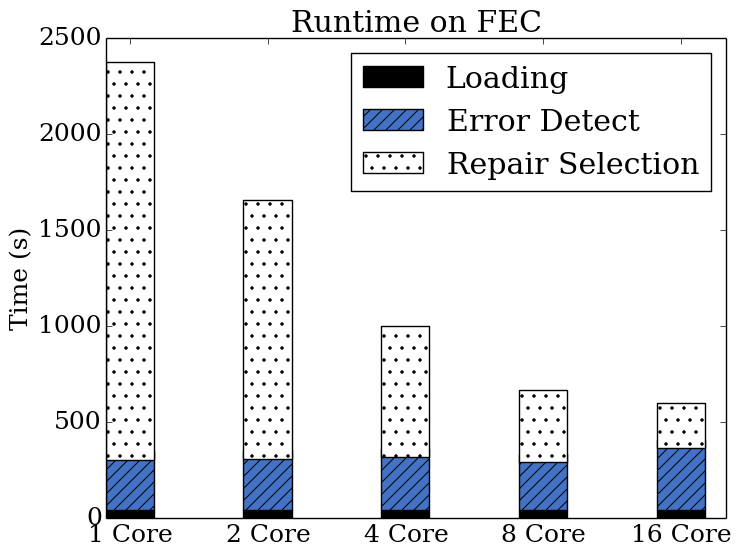
\includegraphics[width=0.8\columnwidth]{exp/runtime.png}
\caption{(A) This plot measures the run-time on a 6M record dataset (1.5GB) grouped by the number of cores on the machine. The repair selection scales but the other steps are not parallelized.\label{exp:runtime}}
\end{figure}

\begin{figure}[t]
\centering
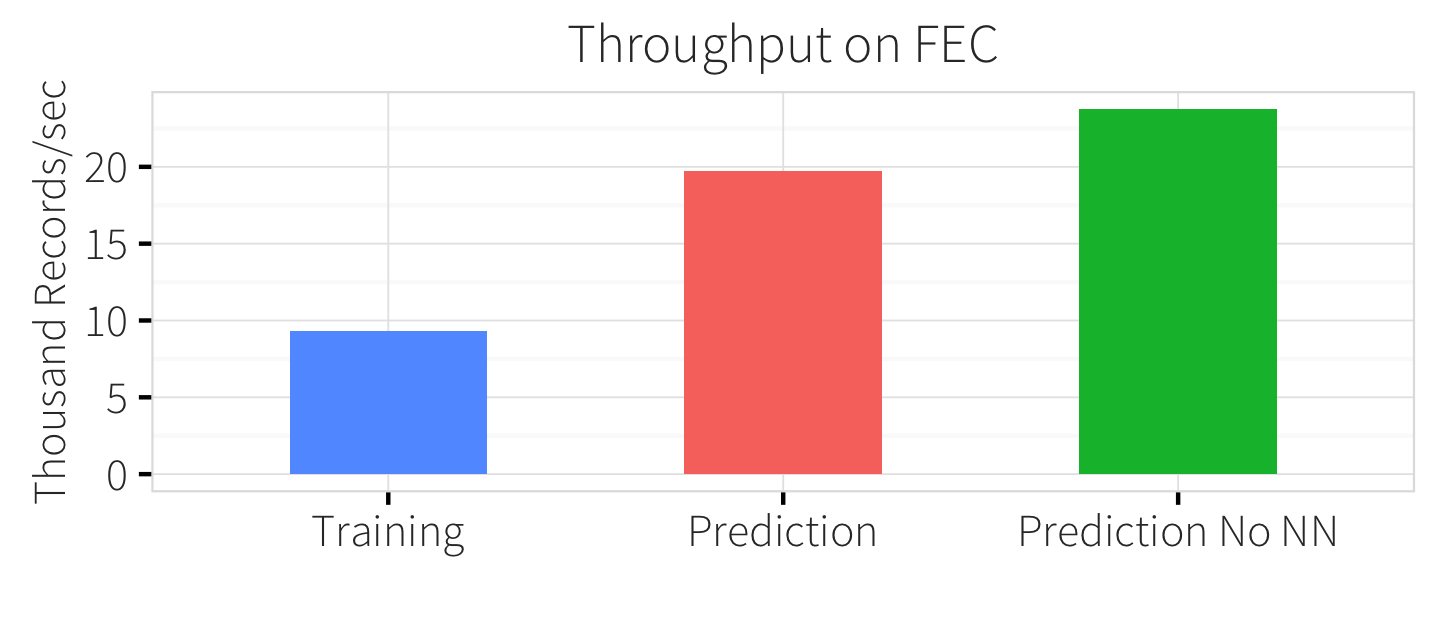
\includegraphics[width=0.8\columnwidth]{exp/runtime2.png}
\caption{We plot the prediction and training throughput for 16-cores. Prediction throughput is much higher than training throughput.\label{exp:tp}}
\end{figure}

\subsection{End-to-End Run Time}
Next, we evaluate the end-to-end wall clock runtime of \sys. We use the FEC dataset since it is the largest. This evaluation includes all of the optimizations for \sys. The FEC dataset is 1.5 GB (about 6M records). 
Figure \ref{exp:runtime} plots the results.
With a single core, \sys takes 2422 seconds in wall-clock time. Of that time, 2072 seconds is spent in repair selection, 306 seconds is spent in error detection, and 44 seconds in loading the dataset.
We can parallelize the repair selection step. We parallelize the inner-loop of the boosting algorithm. On 16-cores, we are able to reduce the runtime of the repair selection to 212 seconds. This constitutes a 9.7x speedup for that step.

It is important to note that this latency is only incurred during training. During prediction, the learned model can be applied, and this process is much faster than training. 
Figure \ref{exp:tp} plots the throughput of \sys.
The number of records that can be processed per second on 16 cores for prediction is 19746 records/second, but during training it is 9316 records/second. One of the key bottlenecks is evaluating the word2vec model for each prediction, and without this model, the throughput increases to 23746 records/second.

\begin{figure}[t]
\centering
 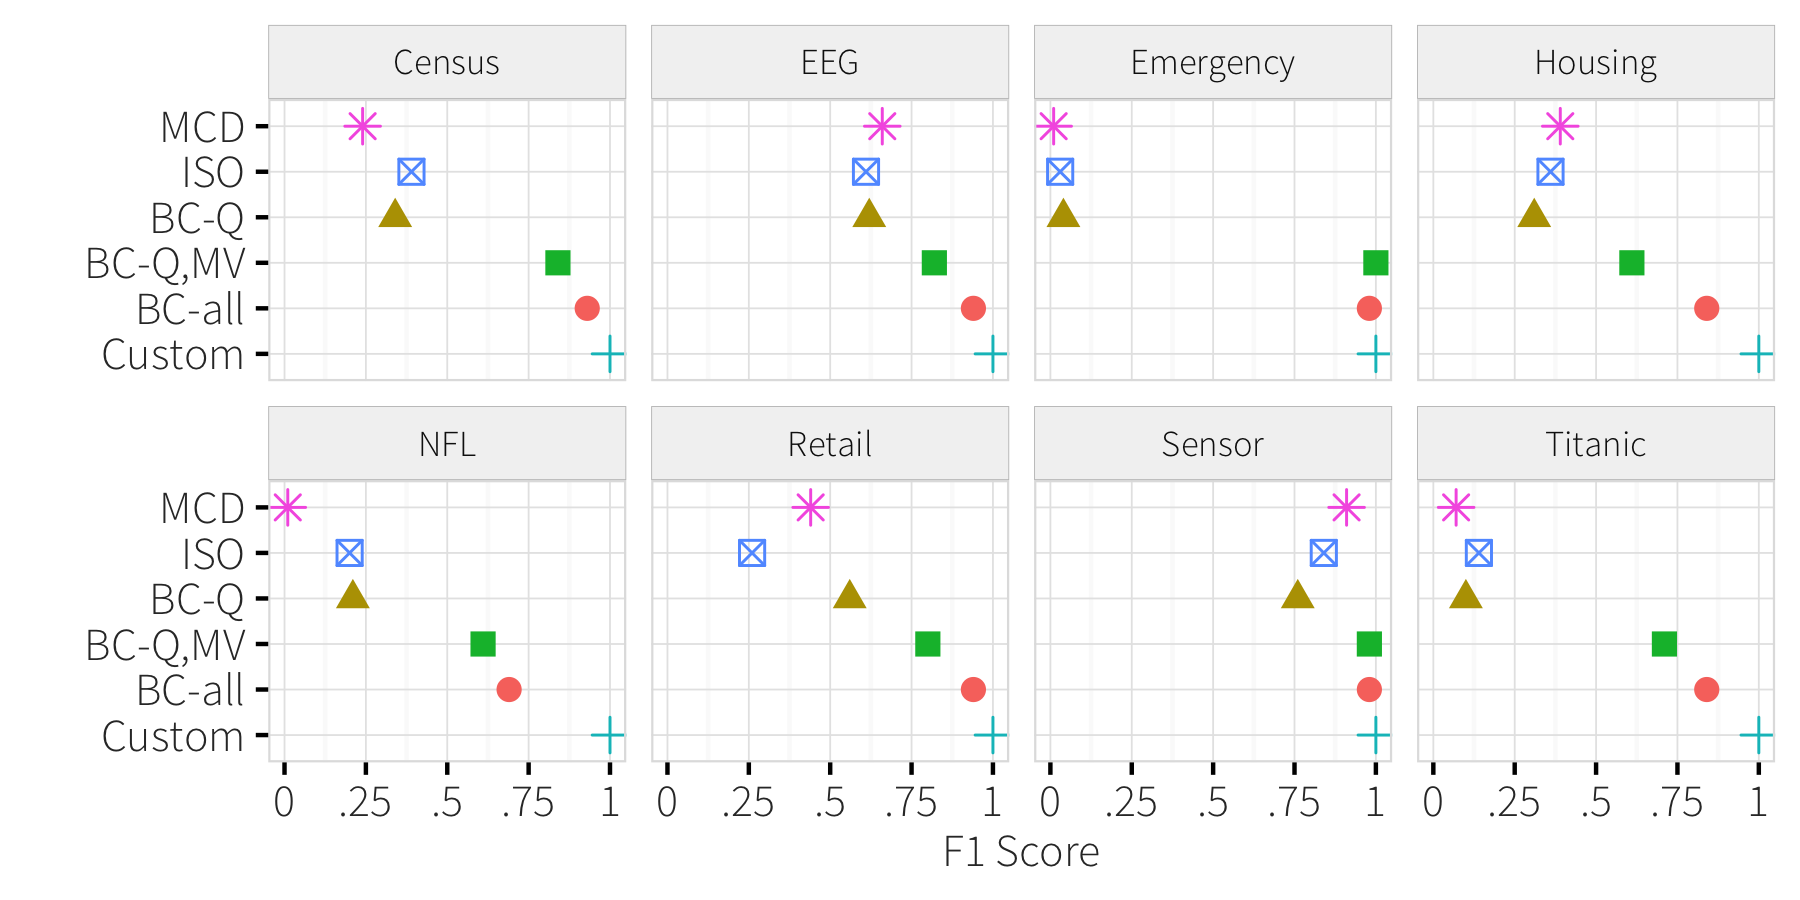
\includegraphics[width=\columnwidth]{exp/daccuracy.png}
 \caption{On 8 Machine Learning competition datasets, we evaluated the F1 accuracy score of different error detection techniques. We compare against Isolation Forest (alone), Minimum Covariance Determinants, and Hand-Written rules. We evaluate \sys using only the Isolation forest for numerical outliers, outliers+missing values, and outliers+missing values+word2vec.
 The final detector in \sys achieves up to 81\% of the accuracy on the competition datasets.
 \label{fig:derror}}
\end{figure}

\begin{figure}[t]
\centering
 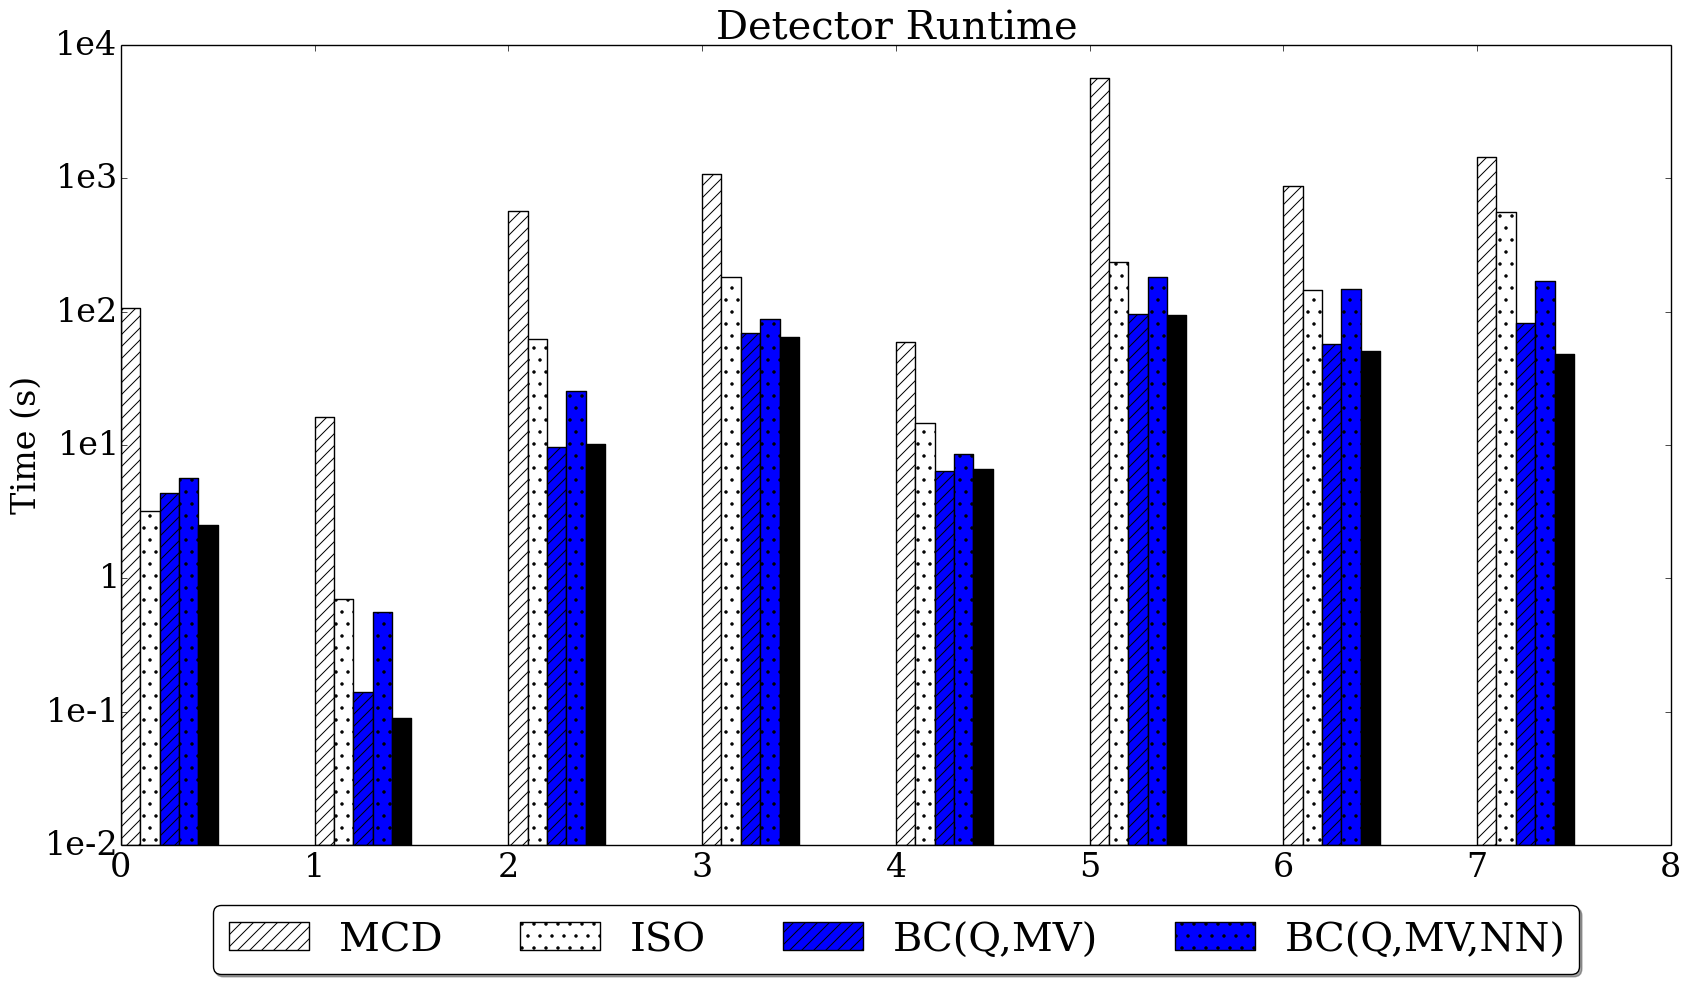
\includegraphics[width=\columnwidth]{exp/druntime.png}
 \caption{On 8 Machine Learning competition datasets, we evaluated the runtime of each of the detection methods. We compare against Isolation Forest, Minimum Covariance Determinants, and Hand-Written rules. While evaluating hand-written rules is certainly faster, \sys is faster in terms of wall-clock time than MCD.
 \label{fig:druntime}}
\end{figure}

\subsection{Micro-Benchmarks}
Next, we evaluate the different components of \sys in terms of accuracy and runtime.

\subsubsection{Detectors}
The first component that we evaluate are the detectors. We design a set of automatic error detectors based on heuristics, statistical criteria, and the word2vec neural network. We first measure its accuracy against hand-written detection scripts, and other quantitative outlier detection techniques (Isolation Forests and Minimum Covariance Determinants).
\sys internally uses an Isolation Forest combined with other error detectors, so we evaluate \sys with and without certain detection modules.
We measure accuracy w.r.t the alternatives with the F1 accuracy measure.

 Figure  \ref{fig:derror} shows that the final detector in \sys achieves up to 81\% of the accuracy of hand-written rules on the competition datasets.
Confirming the results of Abedjan et al.~\cite{DBLP:journals/pvldb/AbedjanCDFIOPST16}, we found that a 
purely quantitative approach does not perform well in comparison to the rule-based approach on these datasets (Isolation Forest alone and MCD).
However, results are significantly improved when combined with heuristics that detect missing values. 
The performance gap is even further reduced when the detector additionally uses a Neural Network to learn how attributes correlate with each other, and detect anomolous correlations.
It is important to emphasize that these datasets represent a very specific domain, i.e., structured training datasets for ML.
The datasets are already in a structured schema and the only thing that an analyst has to worry about is handling inconsistent attribute values.
Presumably these datasets were also previously cleaned and extracted before they were publicly released.
Our initial experiment showed that for this class of datasets, reasonably accurate error detection is possible with minimal supervision and tuning.

 Figure  \ref{fig:druntime} shows the runtime of each of the approaches.
 We found that MCD was a very expensive quantitative error detection approach (orders of magnitude slower).
 This was one of the big motivations for using an isolation forest internally in \sys.
 Of course, rules are faster to evaluate than a learning detector and this gap was on average a factor of 3.
 
 \begin{figure}[t]
\centering
 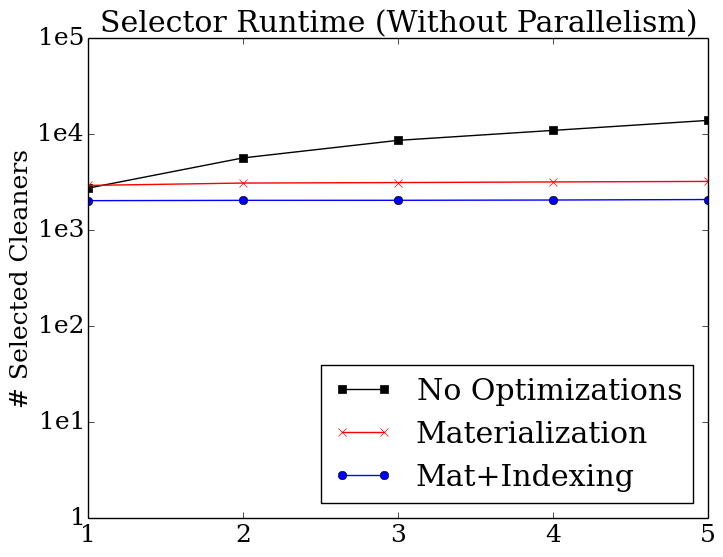
\includegraphics[width=0.9\columnwidth]{exp/opt1.png}
 \caption{This plot (log scale) shows the impact of optimizations on the selector's runtime. Materialization and Indexing allow the algorithm to scale with the number of selected cleaners. Otherwise, the algorithm repeatedly retrains and recleans the same data.
 \label{fig:opt}}
\end{figure}
 
 \subsubsection{Repair Selector Optimizations}
 Next, we evaluate the selector optimizations. We proposed two systems optimizations to the boosting algorithm: (1) materialization, and (2) indexing.
 In this set of experiments, we use FEC dataset and apply no parallelism.
 Figure \ref{fig:opt} plots the runtime of the repair selector as a function of the number of cleaners to select (i.e., B).
 Without any optimization, for $B=1$ the repair selector requires 2754 seconds and for $B=5$ requires 14002 seconds.
 The materialization optimization allows us to pay an up-front cost of creating the view during the first iteration of the algorithm, but saves effort on future iterations.
 For $B=1$ with the materialization optimization, the run time is 2943 seconds.
 For $B=5$ the time is drastically cut down to 3241 seconds.
 In each iteration, the indexing algorithm allows us to more efficiently evaluate the accuracy of a cleaner+classifier pair.
 This reduces the run time at $B=5$ to 2072.
 
 \begin{figure}[t]
\centering
 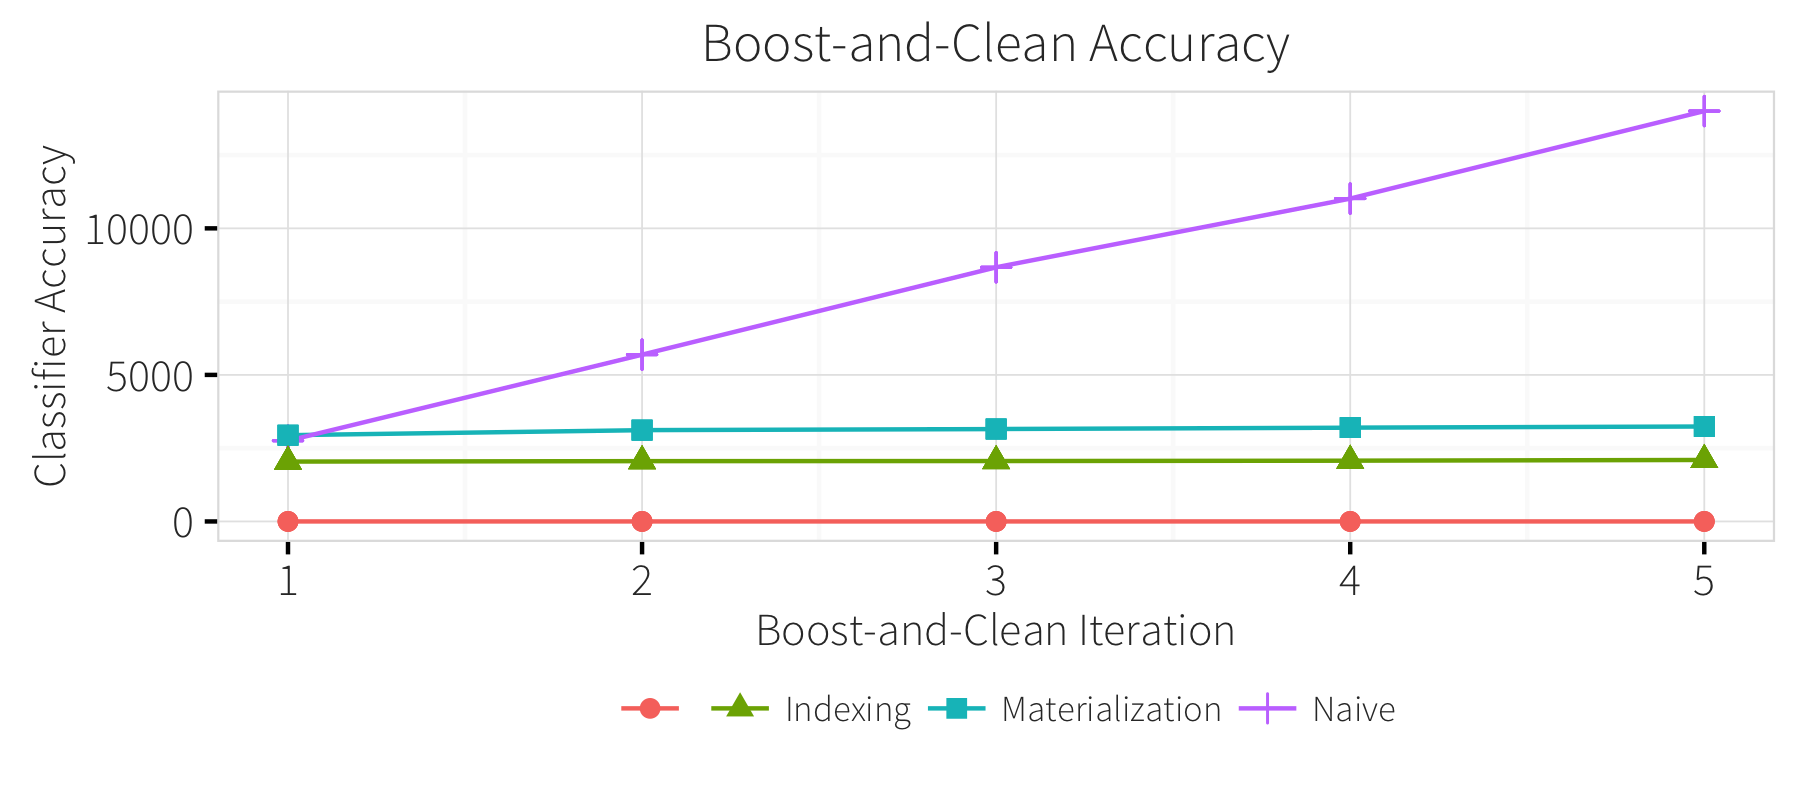
\includegraphics[width=0.9\columnwidth]{exp/learn.png}
 \caption{For three different classification models, we plot the learning curves for the repair selector. Selecting too many cleaners can lead to overfitting.
 \label{fig:learning}}
\end{figure}
 
 \subsubsection{Repair Selector Overfitting}
 One concern with the repair selector is overfitting. We evaluate to what extent, \sys overfits in Figure \ref{fig:learning}, where we plot the learning curves (accuracy as a function of the number of cleaners $B$).
 We try three different classification models, random forests, SVMs, and logistic regression.
 For all of the models we see similar results, where there is an optimal $B$ to select after which \sys overfits.
This is a major concern on small datasets \ewu{How Small?}, but for a sufficiently large dataset with proper test and training evaluation, this can be set through cross-validation. 

\subsubsection{Synthetic Corruptions}

 


